Nguồn: \href{http://dongtac.hncity.org/?THUONG-TIE%CC%81C-MO%CC%A3T-BA%CC%A3C-TRI%CC%81-NHAN&var_mode=calcul&fbclid=IwAR3KZG3yuP5JGpFlxKfT7JIrM8M-7Ihrt9BCZlI1VueWdzuwJqQm2dlqjPU}{Trang Đông Tác }

\begin{figure}
\centering
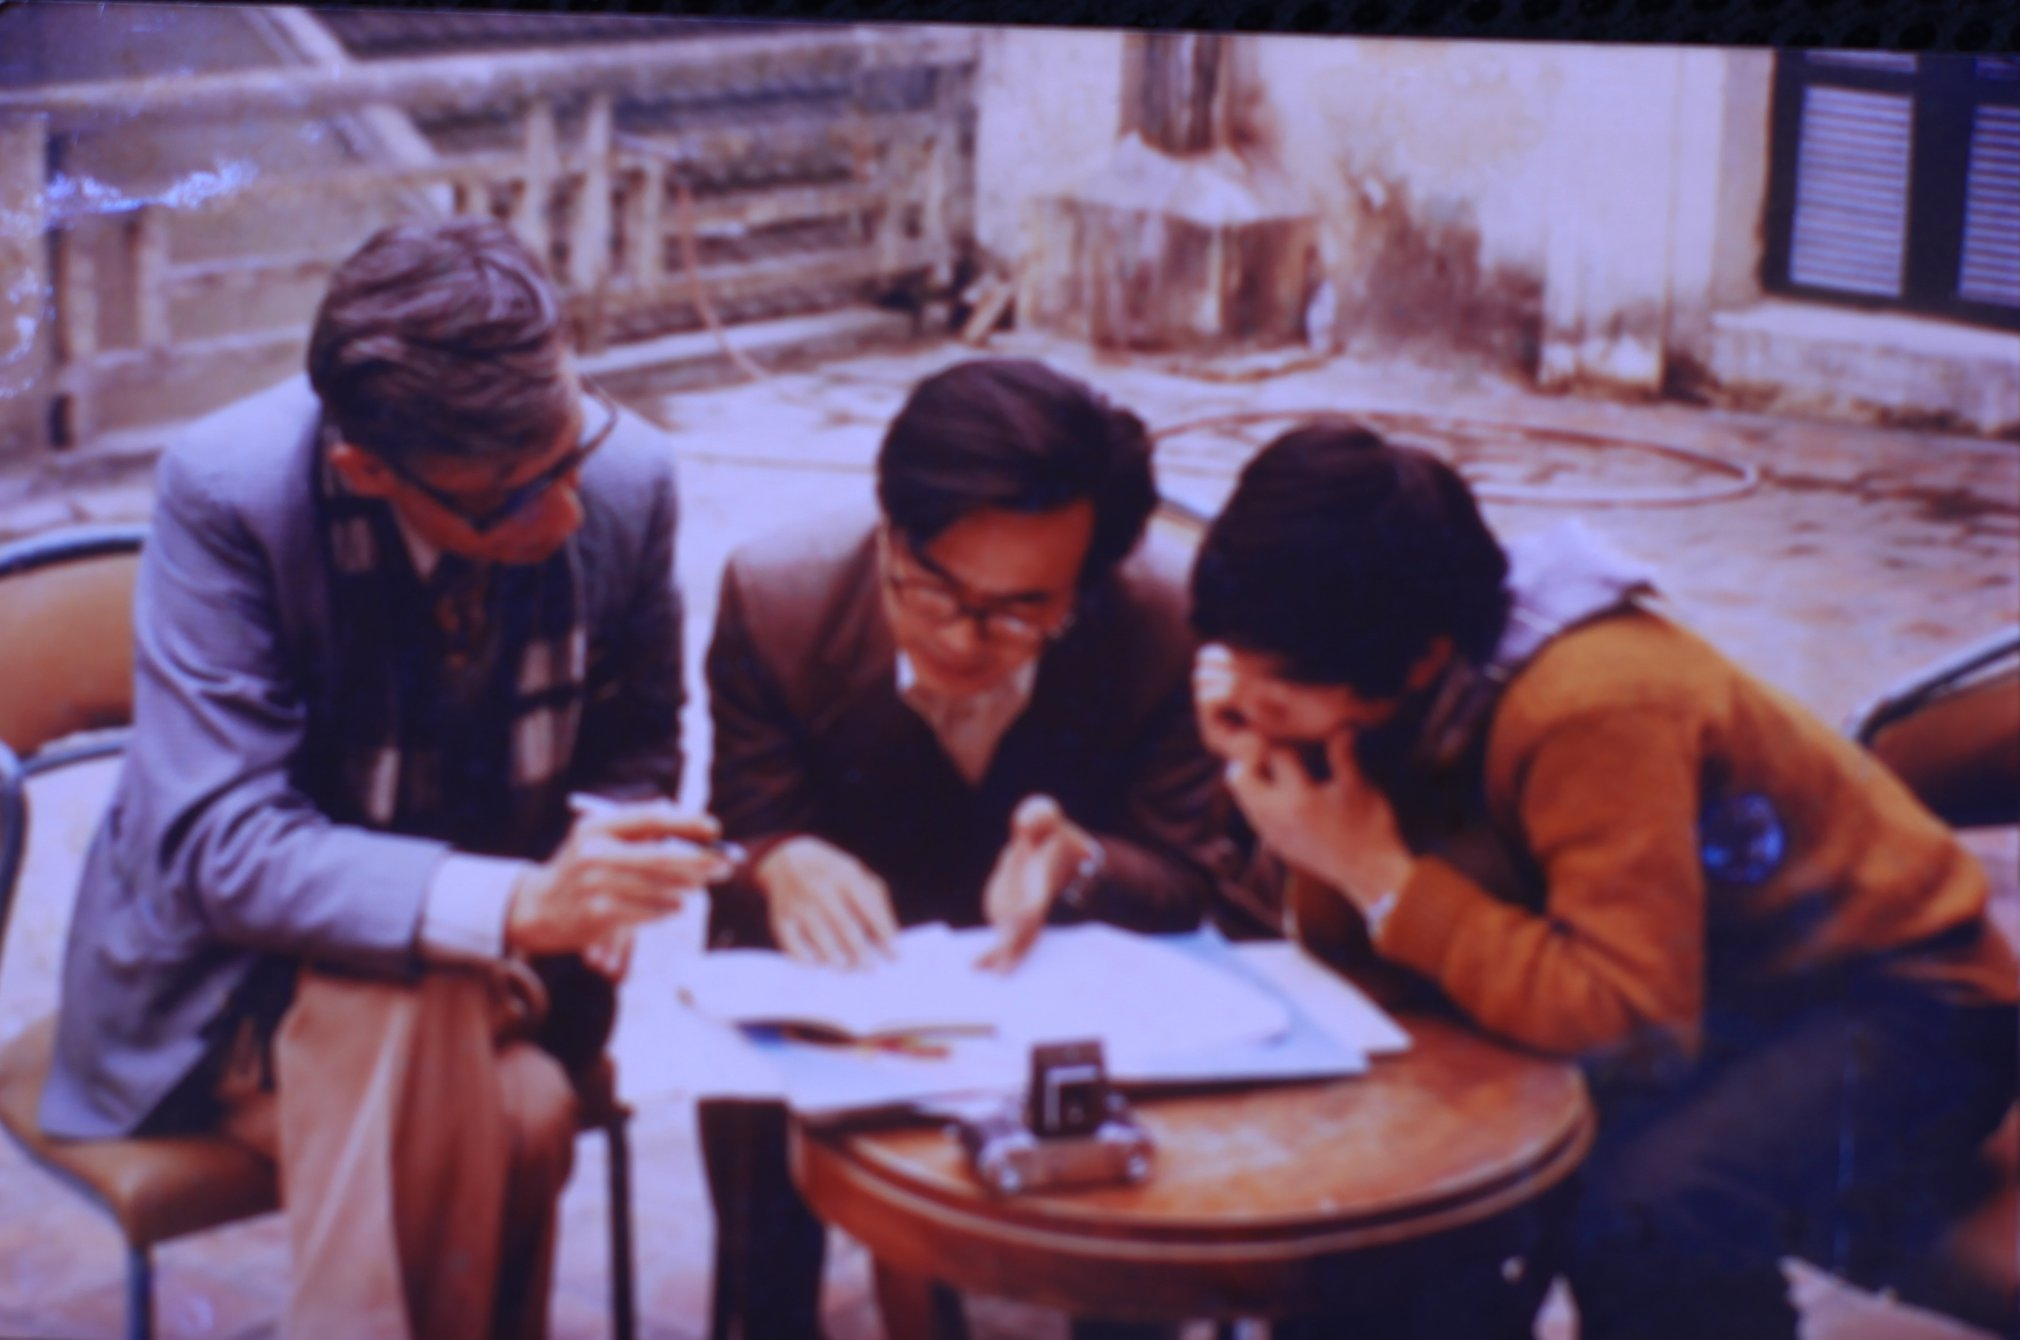
\includegraphics[scale=0.1]{Photos/NguyenChiCong}
\caption{Cuối tháng 2-1979, ngay sau sự kiện TQ xâm lược, tôi tiếp tục đươc tham gia cùng GS H.V. Regemorter và P.Đ. Diệu chuẩn bị kế hoạch đưa ace VN sang Pháp thực tập. Photo (c) CCSTV 1979 tại KS Hoàn Kiếm}
\end{figure}

VÌ SAO MẤT NGỦ

Anh ra đi vào sáng Chúa Nhật hay ngày Thái Dương, và buổi tiễn đưa Anh cuối cùng đã được gia đình thông báo chính thức sẽ tổ chức vào sáng thứ Sáu tức 18-5-2018.

Theo kế hoạch của nhóm Cyclo, lẽ ra chúng tôi phải kết thúc một công việc chung và giao nộp kết quả vào ngày mai 17-5. Nhưng đến phút này, riêng tôi cần xin lỗi các đồng nghiệp vì vẫn chưa thể tập trung suy nghĩ và chỉ đẻ ra ít trang chữ lộn xộn. Cũng trong tâm trạng ngơ ngẩn và sức khoẻ sút kém, tôi đã không thể đến dự buổi giới thiệu cuốn sách tái xuất bản Cái trống thiếc do nhà văn Dương Tường chuyển ngữ.

3h sáng. Không ngủ được, phải ngồi dậy uống trà gừng chống tụt huyết áp. Ngẫm lại mấy ngày qua dù sao cũng đã làm được hai việc có ích để từ giờ có thể cầm bút viết về Anh mà không còn lo sợ quên những điều cần đến tính xác thực. Thứ nhất là tìm ra không ít tư liệu về Anh, thứ hai là cho đăng lại một bài viết của Anh với nhan đề
\href{http://dongtac.hncity.org/?Hai-niem-hanh-phuc-gan-bo-voi-tin-hoc}{Hai niềm hạnh phúc gắn bó với tin học}.

Sau khi lần lượt tìm lại được cả hai chiếc điện thoại: một chiếc để quên trên xe khách và một chiếc bị văng ra do va chạm giao thông, tôi đọc FB và thấy cần nói vài điều với tư cách là một cộng sự rất gần gũi của Anh từ năm 1973 cho mãi đến khi nghỉ hưu. Trước đây vào năm 2007, nhân dịp kỷ niệm 30 năm thành lập Viện Khoa học Tính toán và Điều khiển, theo lời đề nghị của tạp chí Tin học và Đời sống, tôi có viết một hồi ức liên quan đến tập thể các kỹ sư trẻ và Viện trưởng là Anh, một TSKH lúc đó chưa được phong học hàm giáo sư. Toà soạn đã cho đăng liên tiếp ba kỳ, bạn đọc có thể tham khảo ở đây:

Kỳ 1: Chiếc máy vi tính đầu tiên của Việt Nam

Kỳ 2: CÁC THIẾT KẾ MỚI

Kỳ 3: SẢN XUẤT VÀ ỨNG DỤNG

Sinh thời xung quanh Anh, một con người với cuộc đời cực kỳ phong phú, đã từng có biết bao lời bàn tán trái chiều như thói đời vẫn thế. Rồi nay không có Anh đối chất nữa thì càng tăng thêm hiện tượng nói theo cảm tính, đáng tiếc có không ít lời tưởng là tôn vinh mà thực ra làm linh hồn Anh không vui, bởi vì sự chính xác và trung thực vốn là điều Anh quý trọng như bản chất của những trí thức khoa học.

Tối hôm thứ Hai, tôi mở các album trong thư viện nhỏ và thấy ngay hình Anh, nhưng số lượng ít và nội dung có vẻ quan phương, không nói lên những giây phút đời thường của Anh và chúng tôi. Vậy là phải lê đôi chân phù thũng như đeo đá leo lên tận tầng tư để bê xuống mhững túi nhỏ, cứ thế trong ba buổi mất chục lần lên xuống mới tạm yên lòng.

Tôi đã lục tung từng quyển sách trong thư viện lớn rồi lại sang kho mở hết tất cả những thùng giấy phủ đầy bụi bặm. Kết quả là ho rũ rượi và dị ứng toàn thân. Nhưng sau vài lần leo lên leo xuống thì cuối cùng cũng đã hòm hòm tập hợp được vài trăm tấm ảnh cũ kỹ. Ngay tối hôm qua tôi bắt đầu chọn lọc từ đó ra những bức có hình của Anh và gia đình Anh.

Nguyễn Chí Công